\documentclass[10pt,a4paper]{article}
\usepackage{graphicx}
\usepackage{hyperref}
\usepackage{natbib}
\usepackage{booktabs}
\usepackage{makeidx}
\usepackage{tgpagella}
\usepackage[T1]{fontenc}
\usepackage[titletoc]{appendix}
\usepackage[scale=2]{ccicons}

\hypersetup{
    colorlinks=true,       % false: boxed links; true: colored links
    linkcolor=black,          % color of internal links
    citecolor=black,        % color of links to bibliography
    filecolor=magenta,      % color of file links
    urlcolor=black           % color of external links
}

\title{Technical patterns for linking organizations with X-Road}
\author{The Joint X-Road Team}

\makeindex

\begin{document}

\maketitle
\clearpage
\setcounter{tocdepth}{1}
\tableofcontents
\clearpage
\thispagestyle{empty}
\null
\vfill

\begin{center}
This document is licensed under Creative Commons Attribution-NonCommercial-ShareAlike 4.0 International license\\[5mm]

\ccbyncsa\end{center}
\clearpage

\setcounter{section}{0}
\section{Introduction}
\subsection{Goal and structure}
This is document seeks to collect descriptions of architectural patterns that make sense to be used around x-road. The patterns identified are listed in \ref{tab:dir}. 

While all the patterns are usable, no tool is usable for every purpose. Therefore, the patterns are each classified along a set of dimensions allowing for easier navigation and comprehension. The dimensions are defined as follows:
\begin{description}
	\item[Doc\textbackslash Data\textbackslash Service] All of the patterns are particularly suitable for either transmitting documents, data or providing a service. If a patterns is marked as suitable, this means it works well in a given setting and a missing mark means the pattern is not really suitable for a purpose. \index{Document}
	\item[Volume] The volume property denotes the amount of requests a particular pattern is useful for. This is not about absolute numbers but rather relative ones. A pattern marked with \"M\" is suitable for smaller volumes than the one with a \"L\" marking
	\item[Doc direction] Not all patterns are symmetrical in nature. If a document is passed in a transaction, it can move up, down or both ways of the stream. This column indicates, whether the pattern works well for up-stream documents (U), downstream documents (D) or can handle both directions equally well (B). The patterns not suitable for documents are not marked in this column
	 \item[Availability] The systems being integrated might have different availability requirements. If they do, it is important to make sure the availability of one system is not compromised by the availability of the other. This dimension indicates, how the availability of the system in question compares with the one of the integrated system
\end{description}

\begin{table}
	\begin{center}
		\begin{tabular}{p{.5cm}p{3.4cm}p{.9cm}p{.7cm}p{.7cm}p{.8cm}p{.8cm}p{1.2cm}p{1.2cm}}
		\toprule
ID & Pattern & Section & Doc & Data & Service & Volume & Doc direction & Availability \\
\midrule
1 & Straight up xRoad & \ref{section:1} & X &  & S &   & eq \\
2 & Consumer pool & & X & X & X & M & D & $\geq$ \\
3 & Adapterserver & &  & X &  & S &   & eq \\
4 & DVK & & X &  &  & M & B & > \\
5 & Async xRoad provider/consumer & \ref{section:5}  & X & X & X & L & U/D & $\leq$ \\
8 & Gateway to xRoad & \ref{section:8}  &  & X & X & L &  B & $\geq$ \\
9 & Reconciliator  & \ref{section:9} & X & X & X & XL & B & $\leq$ \\
10 & Dead Letter & & X & X &  & XL & U & > \\
11 & Document store &  & X & X &  & L & U & > \\
13 & Read-through cache  & \ref{section:13}  &  & X &  & XL &   & $\gg$ \\
14 & Pub-sub  & \ref{section:14} &  & X &  & L &  & < \\
16 & Aggregated middleware & & X & X & X & XL & U/D & eq \\
\bottomrule
		\end{tabular}
		\caption{Summary of the patterns}
		\label{tab:dir}
	\end{center}
\end{table}

\subsection{Glossary}
\begin{description}
	\item[Consumer]\index{Consumer} The organisation initiating service access. In this document commonly referred to as Alice. The patterns are primarily described from this viewpoint
	\item[Provider]\index{Provider} The organisation receiving service requests. In this document commonly referred to as Bob 
	\item[Information System]\index{Information System} The system at Alice that needs services from Bob or, on the provider side, the system that provides the service
\end{description}

\input{pattern_directory.tex}

\clearpage
\begin{appendices}
\section{X-road overview}
\subsection{Background}
Since very early in the history of computing, smart people have wondered about making systems scalable and maintainable. At a 1968 software engineering conference sponsored by NATO \citep{naur1969software}, the concept of middleware\index{Middleware} was put forth to support the vital system properties of modularity, specification and generality.

The idea of middleware is deceptively simple: to have a unified separation layer between consumers and producers of various services. The main goals of such separation are as follows:
\begin{itemize}
	\item Minimise the number of peer to peer negotiations between parties 
	\item Establish a centralised mechanism for enforcing all sorts of policies like API standards, access rights and so forth
	\item Establish an abstraction layer allowing both parties to live in blissful ignorance of the exact implementation details (and, more importantly, changes of these) of the other. 
\end{itemize}

Typically, such middleware is implemented as a centralised enterprise service bus that faces three main technical obstacles. Firstly, it needs to be all-encompassing to provide value. If some parts of the system manage to sneak the communication past the middleware, alternative methods of policy enforcement need to be put in place, avoidance of which was the point in the first place. Secondly, complexity (and thus cost) of a system follows a S-curve \index{s-curve} in relation to the useful function provided. Thus, a middleware solution servicing 200 requests per second is not twice but about four times more complex than two separate integration solutions servicing 100 requests per second each. Yes, provided sufficient volume, economies of scale kick in but until then, a centralised middleware system is rather costly.

Finally, having a central point where all communication between application layer pass through creates a single point of failure both in terms of operations and development. As such, the middleware needs to fulfil two contradictory requirements: since everything depends on it, the middleware needs to be highly available and very robust and, since, everything depends on it, it must be possible to change often and by numerous parties. 

From the organisational perspective, a question of responsibility arises. Who should take care of the middleware? Most organisations are structured in a way that focuses each of its parts to a certain aspect of running the business. The middleware, however, is involved in everything and is thus difficult to place in a hierarchy. This problem is especially pronounced in case the organisation in question is a democratic country as now the central system must span organisations rather than parts of it. Also, the guiding idea of democracy is to distribute power so its excessive accumulation can be prevented. A centralised middleware solution creates a technical and organisational power nexus that is in direct conflict with this philosophy.

Of course, both technical and organisational issues described can and have been solved. Application of money can overcome many difficulties, some countries have a technologically advanced agency provide middleware services to others etc. In case of Estonia, however, a different approach was taken. Simple lack of money and inability to reach agreement on the placement of the middleware lead to a search of alternatives that culminated with gestation of X-Road. 

\subsection{X-Road architecture}
Instead of a central middleware layer, Estonia developed a system called X-Road, that is distributed in nature and thus is probably best described as a distributed service bus\index{service bus}. Its design is meant to align boundaries on different levels emphasising the fact that it is legally significant organisations exchanging information rather than just information systems. 

X-Road consists of three parts, technical, organisational and legal, none of which is capable of delivering its full value separate from the others. 

From the technical perspective, X-Road consists of identical security servers located at organisational network boundaries and a set of centralised services described in more detail later. Fundamentally the system is a peer to peer system with interoperability being enforced by centrally distributed software rather than standards. Organisationally X-Road is a centrally funded team whose responsibility is the maintenance of central services, development of the security server software and communication with the community running and consuming services using the system. Legally, X-Road is a set of legislative acts issued by the Government of Estonia establishing clear ownership rules around citizen-related data and stating that all government agencies using a legally significant information system must make that information system available to others using X-Road and X-Road only\citep{xteemaarus}. While this setup does not avoid central systems altogether, it seeks to minimise their cost and influence of both development and operations of integration lines. 

Because of the nature of this writing, the following focuses on the technical aspect of X-Road. 

\begin{figure}[ht]
	\begin{center}
		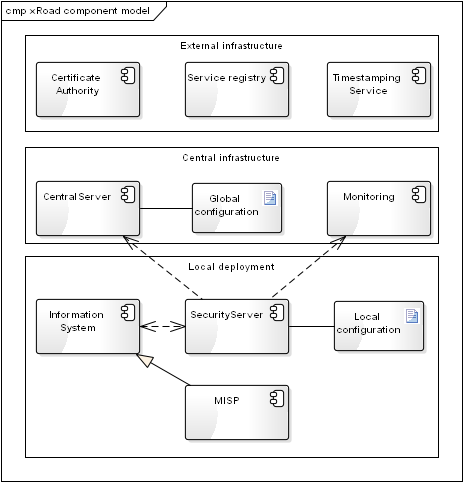
\includegraphics[width=.8\textwidth]{gfx/xroad.png}
		\caption{X-Road component model}
		\label{fig:X-Road}
	\end{center}
\end{figure}

Figure \ref{fig:X-Road} has a component model of a typical X-Road setting where two organisations are exchanging information: one organisation, the service provider, is allowing an other one, the service consumer, to execute queries against a service they run. 

The central part of the system consists of a central server\index{X-Road!Central server}, shared configuration, a service registry and a certificate authority\index{Certificate Authority}. A central server has two main functions. From one hand, it is the management and distribution vehicle for shared configuration. From the other, it collects statistics and various feedback from the locally deployed security servers. No communication actually passes through the central server - it could disappear from the network for hours without any impact on X-Road service availability. Shared configuration is, as the name implies, configuration that is shared between the security servers. It includes both low level network configuration parameters required for communication between security servers and information related to the certificate authority. 

In order to make the services provided truly useful, a discovery mechanism is needed. In case of X-Road, there are two of those. Firstly, all services are (manually) reported to a central service registry\index{X-Road!Service registry} along with documentation to facilitate manual searches. Secondly, the Security Servers are able to respond to meta-requests about services provided. 

Finally, the certificate authority is the key part of the way authentication and authorisation happens on X-Road. Every agency is issued a digital certificate that is used for both encryption of all communications and assuring only authorised agencies have access to services. In addition to the agency certificates, server certificates are issued to allow for separation between server and organisation identities. The latter is useful in co-hosting and service migration scenario.

For a service provider, the key part of the system is a Security Server\index{X-Road!Security Server}. It performs the function of a gatekeeper acting as the the main point of contact for accessing the information system (IS) providing the actual business service. In terms of service consumption, the security server is almost transparent: an external system could access the services directly as the Security Server only adds certain metadata headers about the requesting party. At least as long as the access rules have been configured to allow access. If that is not the case, the gate is shut and the service is not available. In addition to preventing unauthorised access and encrypting the traffic, the security server reports usage statistics to the central server and provides utility functions like offering a list of services it knows about and supplying service monitoring hooks. Both in front and behind the security server, load balancers might be located for balancing load and increasing availability. 

In addition to blocking unauthorised access and securing the communication channel, the security server also ensures the irrefutability of requests and responses by digitally signing the requests and responses and sending hashes of all communication to the central server. The digital signatures are legal under Estonian law and are equal to the official stamp of the organisation.

On the side of the service consumer, there is another instance of the Security Server. In this position it acts as a "stub" towards the local information system. For the latter, it would seem that the Security Server is providing answers to all the queries while, in fact, it performs lookup for the precise network location of its counterpart, executes the query requested and returns the result. In addition to using the service from the information system, it is also possible to consume X-Road services via a simple auto-generated user interface using the MISP\index{X-Road!MISP}\footnote{Mini Information System Portal} component. Since the service descriptions are machine-readable, they can be used to generate user interfaces for entering basic request parameters and displaying the response. The resulting user experience, depending on service description quality and sophistication of the generating software, is far from smooth but is sufficient for consumption of simple services or debugging of more complex ones.

Thus the pair of security servers form a semi-transparent secure layer between the two information systems. This means that it would in theory be possible for one system to execute all the service requests directly against the other system without the Security Servers. To do this, the two organisations would need to establish a contractual relationship about the data exchanged, agree upon a channel security mechanism, agree and establish a credential exchange process, agree upon service monitoring, communication protocols, security incident response and all the nitty gritty it takes for organisations to talk to each other. Such a process might be fine for a few integration points but would rapidly become cumbersome as the number of partners grows. X-Road allows to scale an otherwise non-scalable set of peer to peer relationships between organisations. 

\subsection{Summary}
In summary, this is what X-Road offers:

\begin{enumerate}
	\item Authentication of agencies for computer-to-computer interaction
	\item Channel protection for computer-to-computer interaction
	\item Fine-grained service access control for the authenticated agencies
	\item Irrefutability of requests and responses
	\item A service lookup and discovery mechanism   
\end{enumerate}

In addition, it is as important to note, what X-Road \emph{does not} do. 

Firstly, X-Road does not offer any end-user capabilities other than the loosely attached MISP portal. By design, X-Road is a mechanism for organisations to exchange information and thus its trust framework is about organisations trusting or not trusting each other. Therefore, the responsibility to offer user interaction and make sure that can only be accessed by authorised users, lies with the organisations using X-Road and not X-Road itself.

X-Road also does not offer any load balancing or availability-related services. It merely knows a list of addresses a service is available at. Making sure that service is indeed available at these addresses is the sole responsibility of the service provider. This of course leads to clear issues with agreeing upon service levels - i.e. what is the expected availability of a service and what happens if these expectations are not met. X-Road in itself does not offer a mechanism for neither communicating nor enforcing any service levels. 

This brief overview can not hope to encompass all the complexity related to X-Road, least because it is being constantly developed. The best resource for up to date detailed technical information on the inner workings of X-Road is the Security Server User's Guide \cite{xroadmanual}. 
\end{appendices}
\clearpage

\bibliographystyle{plain}
\bibliography{xroad_distilled} 

\end{document}